Here we outline the algorithm currently implemented in the code.  Our
starting point for this description are the series of papers describing
the development of the algorithm:
\begin{itemize}
\item {\em Low Mach Number Modeling of Type Ia
  Supernovae. I. Hydrodynamics,} A. S. Almgren, J. B. Bell, 
  C. A. Rendleman, \& M. Zingale 2006, ApJ, 637, 922 (henceforth
  paper I)
\item {\em Low Mach Number Modeling of Type Ia Supernovae. II. Energy
  Evolution,} A. S. Almgren, J. B. Bell, C. A. Rendleman, \& M. Zingale
  2006, ApJ, 649, 927 (henceforth paper II)
\item {\em Low Mach Number Modeling of Type Ia Supernovae. III. Reactions,}
  A. S. Almgren, J. B. Bell, A. Nonaka, \& M. Zingale
  2008, ApJ, 684, 449 (henceforth paper III)
\item {\em Low Mach Number Modeling of Type Ia Supernovae. IV. White Dwarf Convection,}
  M. Zingale, A. S. Almgren, J. B. Bell, A. Nonaka, \& S. E. Woosley
  2009, ApJ, 704, 196 (henceforth paper IV)
\item {\em MAESTRO: An Adaptive Low Mach Number Hydrodynamics Algorithm for Stellar
  Flows,} A. Nonaka, A. S. Almgren, J. B. Bell, M. J. Lijewski, C. M. Malone,
  \& M. Zingale 2009, submitted to SIAM J. Sci. Comput. 
  (henceforth ``the multilevel paper'')
\end{itemize}
We also carry over some ideas from our small-scale low Mach number algorithm
for astrophysical flows:
\begin{itemize}
\item {\em Adaptive Low Mach Number Simulations of Nuclear Flames,}
J. B. Bell, M. S. Day, C. A. Rendleman, S. E. Woosley, \& M. Zingale
2004, JCP, 195, 2, 677 (henceforth BDRWZ)
\end{itemize}

\section{Changes Between Paper 3 and Paper 4}
\begin{enumerate}
\item We defined the mapping of data between a 1D radial array and the 3D Cartesian
grid for spherical problems (which we improve upon in the multilevel paper).
\item We update $T$ after the call to {\bf React State}.
\item We have created a {\tt burning\_cutoff\_density}, where the burning does
not happen below this density.  It is presently set to {\tt base\_cutoff\_density}.
\item Use corner coupling in advection.
\item We use {\tt use\_tfromp} to update temperature using $T=T(\rho,X_k,p_0)$ rather 
than $T=T(\rho,h,X_k)$.
\item For spherical problems, we have changed the discretization of 
$\Ubt\cdot\nabla p_0$ in the enthalpy update to 
$\nabla\cdot(\Ubt p_0) - p_0\nabla\cdot\Ubt$.
\item In paper III we discretized the enthalpy evolution equation in
terms of $T$.  Since then we have discovered that 
discretizing the enthalpy evolution in perturbational form, $(\rho h)'$,
leads to better numerical properties.  We use {\tt enthalpy\_pred\_type = 1}.
This is more like paper II.
\item We have turned off the evolution of $h$ above the atmosphere and instead
compute $h$ with the EOS using {\tt do\_eos\_h\_above\_cutoff = TRUE}.
\end{enumerate}
\section{Changes Between Paper 4 and the Multilevel Paper}
See the multilevel paper for the latest.
\section{Changes Between Papers 4.5 and Paper 5}
\begin{enumerate}
\item Added rotation.
\end{enumerate}
\section{Changes Between Paper 5 and XRB Paper}
\begin{enumerate}
\item We have added thermal diffusion, controlled by {\tt use\_thermal\_diffusion},
{\tt temp\_diffusion\_formulation}, and {\tt thermal\_diffusion\_type}.
\item We added the volume discrepancy term to the velocity constraint equation,
controlled by the input parameter, {\tt dpdt\_factor}.
\end{enumerate}

%-----------------------------------------------------------------------------
% Future Considerations
%-----------------------------------------------------------------------------

\section{Future Considerations}

\begin{itemize}

\item Should we use a predictor-corrector for updating the full-state density?
Specifically, after calling {\bf Correct Base}, should we do a full-state density 
advance and {\bf Correct Base} using the more accurate estimate of $\rho_0^{n+1}$?

\end{itemize}

%-----------------------------------------------------------------------------
% Time Advancement Algorithm
%-----------------------------------------------------------------------------

\section{Time Advancement Algorithm}\label{Sec:Time Advancement Algorithm}
Here are changes to the algorithm from the multilevel paper description.
The initialization has also been included with more detail than was given in paper III.
\subsection{Volume Discrepancy Changes}
\begin{itemize}
\item In {\bf Step 2B}, to compute $w_0$, we need to account for the volume discrepancy
term by computing $p_{\rm EOS} = \overline{p(\rho,h,X_k)^n}$.
\item In {\bf Step 3}, the MAC projection should account for the volume discrepancy term:
\begin{equation}
\nabla \cdot \left(\beta_0^n \uadvone\right) = 
\beta_0^n \left\{ \left(S^{\nph,\star\star} - \overline{S^{\nph,\star\star}}\right)
+ \frac{f}{\gammabar^n p_0^n}
\left[\frac{p(\rho,h,X_k)^n - \overline{p(\rho,h,X_k)^n}}{\Delta t^n}\right]\right\}.
\end{equation}
\item In {\bf Step 6B}, to compute $w_0$, we need to account for the volume discrepancy
term by computing $p_{\rm EOS} = \left[\overline{p(\rho,h,X_k)^n} + \overline{p(\rho,h,X_k)^{n+1,\star}}\right]/2$.
\item In {\bf Step 7}, the MAC projection should account for the volume discrepancy term:
\begin{equation}
\nabla \cdot \left(\beta_0^{\nph,\star} \uadvtwo\right) = \beta_0^{\nph,\star}\left\{\left(S^{\nph,\star} - \overline{S^{\nph,\star}}\right) + \frac{f}{\overline{\Gamma_1^{\nph,\star}} p_0^{\nph,\star}} \left[\frac{p(\rho,h,X_k)^{\nph,\star} - \overline{p(\rho,h,X_k)^{\nph,\star}}}{\Delta t^n}\right]\right\},
\end{equation}
where $p(\rho,h,X_k)^{\nph,\star} = \left[p(\rho,h,X_k)^n +p(\rho,h,X_k)^{n+1,\star}\right]/2$.
\item In {\bf Step 11}, the approximate projection should account for the volume
discrepancy term:
\begin{equation}
\nabla \cdot \left(\beta_0^{\nph} \Ubt^{n+1} \right)  = \beta_0^{\nph}\left\{  \left(S^{n+1} - \overline{S^{n+1}} \right)
+ \frac{f}{\overline{\Gamma_1^{n+1}} p_0^{n+1}}
\left[\frac{p(\rho,h,X_k)^{n+1} - \overline{p(\rho,h,X_k)^{n+1}}}{\Delta t^n}\right]\right\}.
\end{equation}
\end{itemize}
\subsection{Thermal Diffusion Changes}
Immediately after {\bf Step 4H}, diffuse the enthalpy through 
a time interval of $\dt$.  First, define $(\rho h)^{(1a),\star} = (\rho h)^{(2),\star}$.  
We recompute $(\rho h)^{(2),\star}$ to account for thermal diffusion.  Here we begin
with the enthalpy equation, but consider only the 
diffusion terms,
\begin{equation}
\frac{\partial (\rho h)}{\partial t} = \nabla\cdot\kth\nabla T.
  \end{equation}
We can recast this as an enthalpy-diffusion equation by applying the
chain-rule to $h(p_0,T,X_k)$,
\begin{equation}
\nabla h = h_p \nabla p_0 + c_p \nabla T + \sum_k \xi_k \nabla X_k \enskip ,
\end{equation}
giving
\begin{equation}
  \frac{\partial (\rho h)}{\partial t}  = 
 \nabla\cdot \frac{\kth}{c_p}\nabla h -  
 \sum_k \nabla\cdot \frac{\xi_k \kth}{c_p}\nabla X_k -
 \nabla\cdot \frac{h_p \kth}{c_p}\nabla p_0.
  \end{equation}
Compute $\kth^{(1)}, c_p^{(1)}$, and $\xi_k^{(1)}$ from $\rho^{(1)}, T^{(1)}$, and $X_k^{(1)}$ as inputs to the equation of state.  The update is given by
\begin{eqnarray}
(\rho h)^{(2),\star} &=& (\rho h)^{(1a),\star} + \frac{\dt}{2}\nabla\cdot\left(\frac{\kth^{(1)}}{c_p^{(1)}}\nabla h^{(2),\star} + \frac{\kth^{(1)}}{c_p^{(1)}}\nabla h^{(1)}\right)\nonumber\\
&&- \frac{\dt}{2}\sum_k\nabla\cdot\left(\frac{\xi_k^{(1)}\kth^{(1)}}{c_p^{(1)}}\nabla X_k^{(2),\star} + \frac{\xi_k^{(1)}\kth^{(1)}}{c_p^{(1)}}\nabla X_k^{(1)}\right)\nonumber\\
&&- \frac{\dt}{2}\nabla\cdot\left(\frac{h_p^{(1)}\kth^{(1)}}{c_p^{(1)}}\nabla p_0^{n+1,\star} + \frac{h_p^{(1)}\kth^{(1)}}{c_p^{(1)}}\nabla p_0^{n}\right),
\end{eqnarray}
which is numerically implemented as a diffusion equation for $h^{(2),\star}$,
\begin{eqnarray}
\left(\rho^{(2),\star} - \frac{\dt}{2}\nabla\cdot\frac{\kth^{(1)}}{c_p^{(1)}}\nabla\right)h^{(2),\star} &=& (\rho h)^{(1a),\star} + \frac{\dt}{2}\nabla\cdot\frac{\kth^{(1)}}{c_p^{(1)}}\nabla h^{(1)}\nonumber\\
&&- \frac{\dt}{2}\sum_k\nabla\cdot\left(\frac{\xi_k^{(1)}\kth^{(1)}}{c_p^{(1)}}\nabla X_k^{(2),\star} + \frac{\xi_k^{(1)}\kth^{(1)}}{c_p^{(1)}}\nabla X_k^{(1)}\right)\nonumber\\
&&- \frac{\dt}{2}\nabla\cdot\left(\frac{h_p^{(1)}\kth^{(1)}}{c_p^{(1)}}\nabla p_0^{n+1,\star} + \frac{h_p^{(1)}\kth^{(1)}}{c_p^{(1)}}\nabla p_0^{n}\right),
\end{eqnarray}

Immediately after {\bf Step 8H}, diffuse the enthalpy through a time interval of 
$\dt$.  First, define $(\rho h)^{(1a)} = (\rho h)^{(2)}$.  We recompute $(\rho h)^{(2)}$ to 
account for thermal diffusion.  Compute $\kth^{(2),\star}, c_p^{(2),\star}$, and 
$\xi_k^{(2),\star}$, from $\rho^{(2),\star}, T^{(2),\star}$, and $X_k^{(2),\star}$ as inputs to 
the equation of state.  The update is given by
\begin{eqnarray}
(\rho h)^{(2)} &=& (\rho h)^{(1a)} + \frac{\dt}{2}\nabla\cdot\left(\frac{\kth^{(2),\star}}{c_p^{(2),\star}}\nabla h^{(2)} + \frac{\kth^{(1)}}{c_p^{(1)}}\nabla h^{(1)}\right)\nonumber\\
&&- \frac{\dt}{2}\sum_k\nabla\cdot\left(\frac{\xi_k^{(2),\star}\kth^{(2),\star}}{c_p^{(2),\star}}\nabla X_k^{(2)} + \frac{\xi_k^{(1)}\kth^{(1)}}{c_p^{(1)}}\nabla X_k^{(1)}\right)\nonumber\\
&&- \frac{\dt}{2}\nabla\cdot\left(\frac{h_p^{(2),\star}\kth^{(2),\star}}{c_p^{(2),\star}}\nabla p_0^{n+1} + \frac{h_p^{(1)}\kth^{(1)}}{c_p^{(1)}}\nabla p_0^{n}\right),
\end{eqnarray}
which is numerically implemented as a diffusion equation for $h^{(2)}$.
\begin{eqnarray}
\left(\rho^{(2)} - \frac{\dt}{2}\nabla\cdot\frac{\kth^{(2),\star}}{c_p^{(2),\star}}\nabla\right)h^{(2)} &=& (\rho h)^{(1a)} + \frac{\dt}{2}\nabla\cdot\frac{\kth^{(1)}}{c_p^{(1)}}\nabla h^{(1)}\nonumber\\
&&- \frac{\dt}{2}\sum_k\nabla\cdot\left(\frac{\xi_k^{(2),\star}\kth^{(2),\star}}{c_p^{(2),\star}}\nabla X_k^{(2)} + \frac{\xi_k^{(1)}\kth^{(1)}}{c_p^{(1)}}\nabla X_k^{(1)}\right)\nonumber\\
&&- \frac{\dt}{2}\nabla\cdot\left(\frac{h_p^{(2),\star}\kth^{(2),\star}}{c_p^{(2),\star}}\nabla p_0^{n+1} + \frac{h_p^{(1)}\kth^{(1)}}{c_p^{(1)}}\nabla p_0^{n}\right),
\end{eqnarray}


%-----------------------------------------------------------------------------
% graphical flowcharts
%-----------------------------------------------------------------------------
\begin{figure}[tb]
\centering
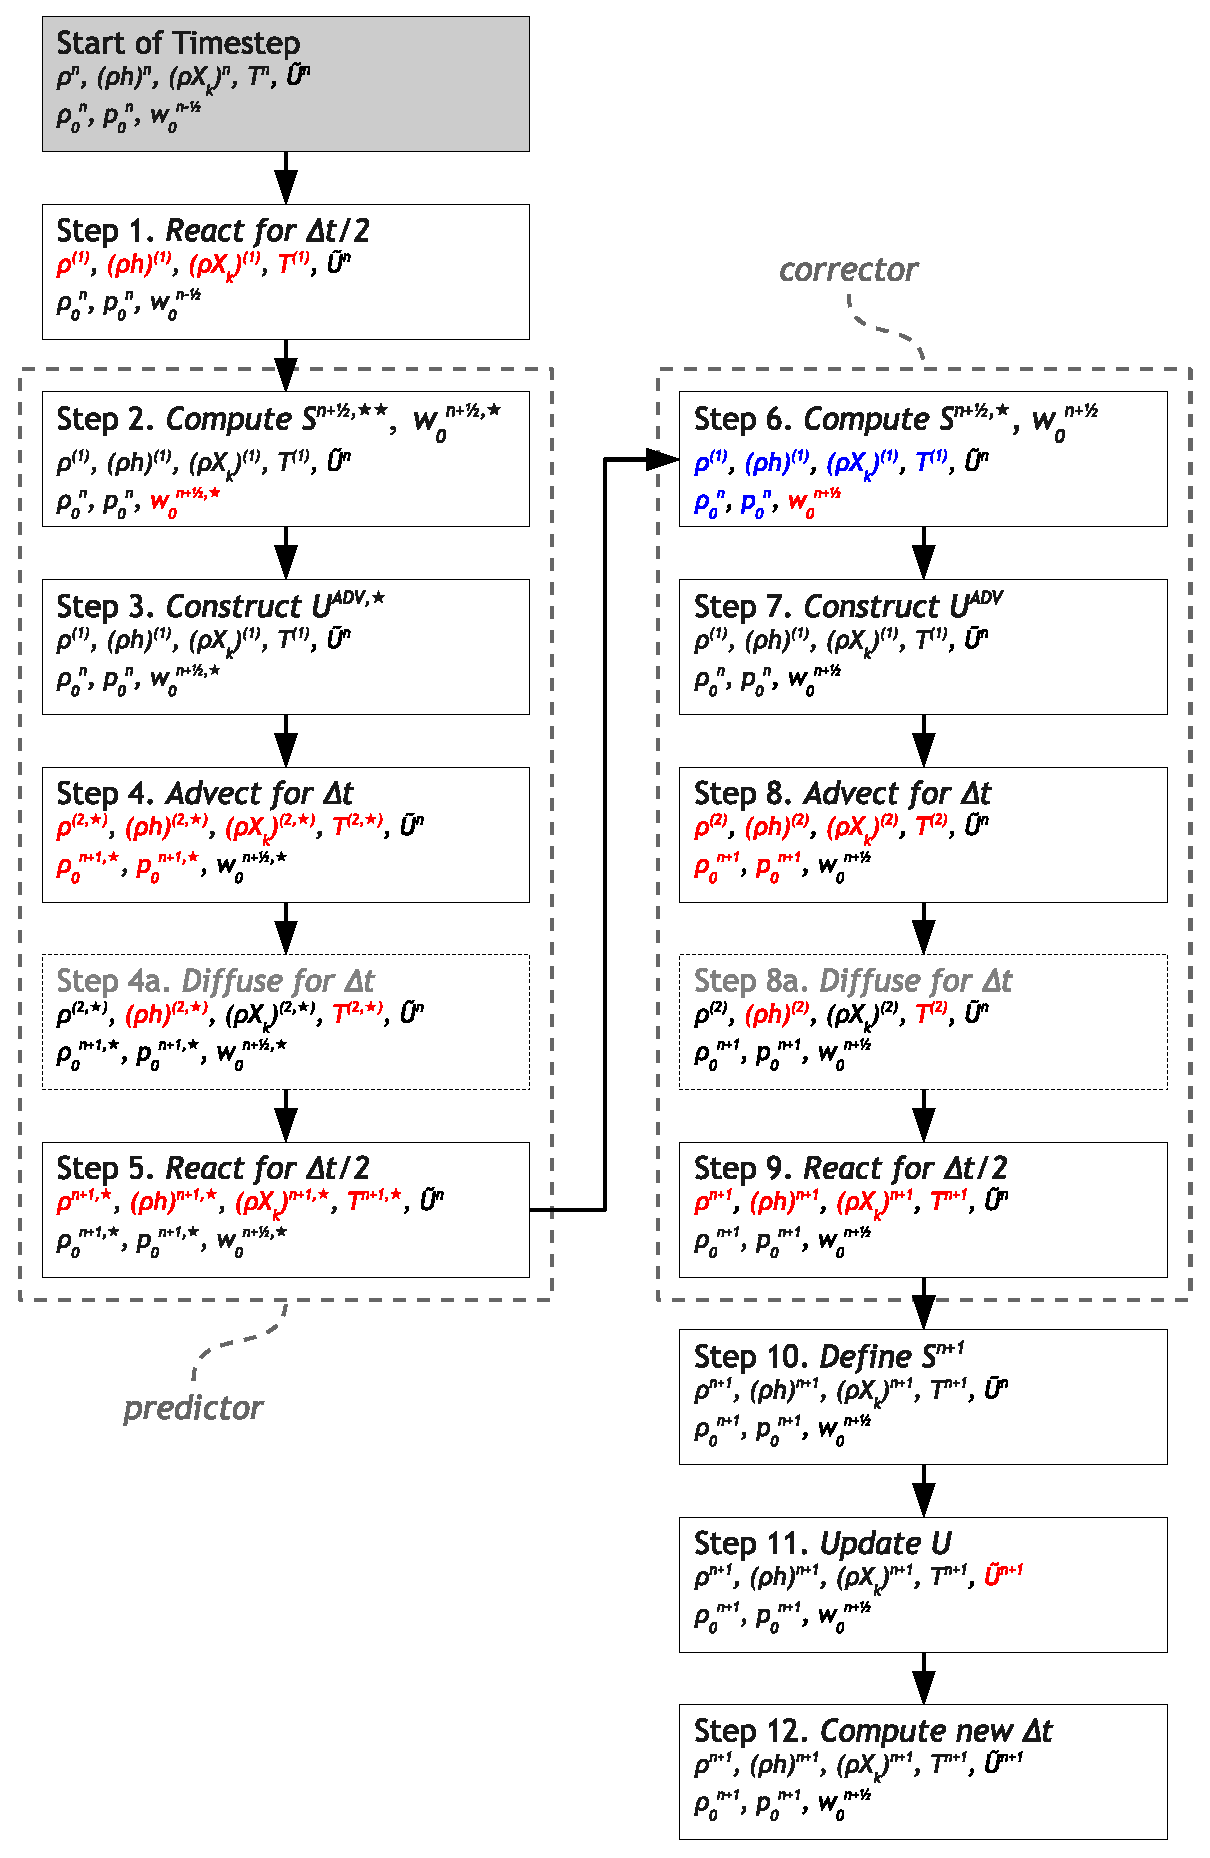
\includegraphics[scale=0.6]{\flowfigpath/flowchart}
\caption{\label{Fig:flowchart} A flowchart of the algorithm.  The
  thermodynamic state variables, base state variables, and local velocity are
  indicated in each step.  Red text indicates that quantity was
  updated during that step.  The predictor-corrector steps are
  outlined by the dotted box.  The blue text indicates state
  variables that are the same in {\bf Step 6} as they are in
  {\bf Step 2}, i.e., they are unchanged by the predictor steps.}
\end{figure}
%%%%%%%%%%%%%%%%%%%%%%%%%%%%%%%%%
%%%%%%%%%%%%%%%%%%%%%%%%%%%%%%%%%
\begin{figure}[tb]                                               
\centering
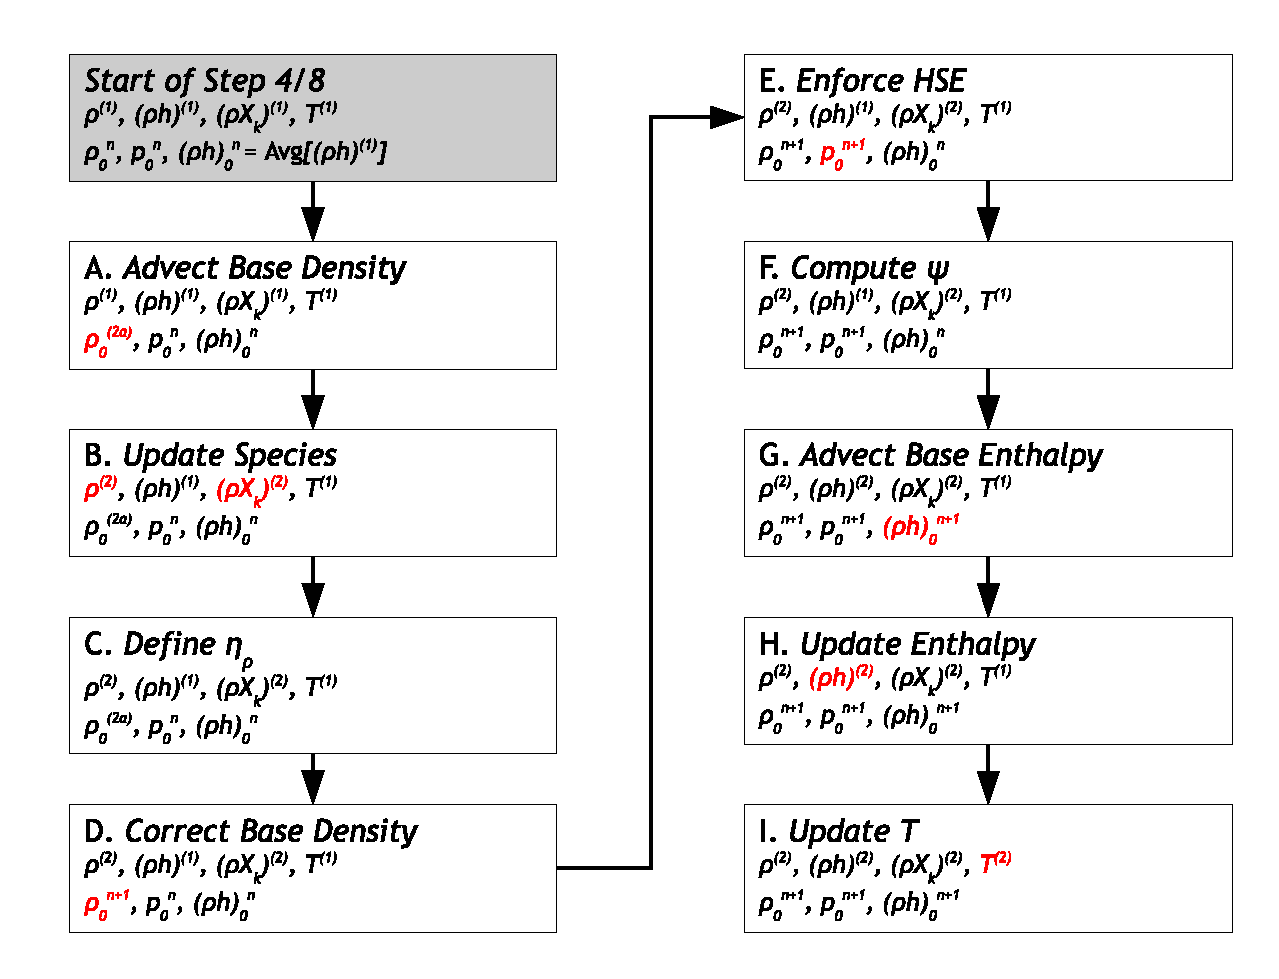
\includegraphics[scale=0.6]{\flowfigpath/flowchart_4_8}
\caption{\label{Fig:flowchart48}
A flowchart for {\bf Steps 4} and {\bf 8}.  The thermodynamic state variables
and base state variables are indicated in each step.  Red text indicates that q\
uantity
was updated during that step.  Note, for {\bf Step 4}, the updated
quantities should also have a $\star$ superscript, e.g., {\bf Step 8I} defines
$T^{(2)}$ while {\bf Step 4I} defines $T^{(2),\star}$ .}
\end{figure}


%-----------------------------------------------------------------------------
% Initialization
%-----------------------------------------------------------------------------

\section{Initialization}\label{Sec:Initialization}

We start each calculation with user-specified initial values for
$\rho$, $X_k$ and $T,$ as well as an initial background state.  In
order for the low Mach number assumption to hold, the initial data
must be thermodynamically consistent with the initial background
state.  In addition, the initial velocity field must satisfy an
initial approximation to the divergence constraint.  We use an iterative
procedure to compute both an initial right-hand-side for the
constraint equation and an initial velocity field that satisfies
the constraint.  The user specifies the number of iterations,
$N_{\rm iters}^{S},$ in this first step of the initialization procedure.

The initial perturbational pressure also needs to be determined for
use in {\bf Steps 3}, {\bf 7}, and {\bf 11}. 
This is done through a second iterative procedure which follows the
time advancement algorithm as described in {\bf Steps 1-11} in 
\S \ref{Sec:Time Advancement Algorithm}.  
The user specifies the number of iterations, 
$N_{\rm iters}^{\pi},$ in this second step of the initialization procedure.
The details for both iterations are given below.\\

%--------------------------------------------------------------------------
% STEP 0
%--------------------------------------------------------------------------
\noindent {\bf Step 0.} {\em Initialization}

First, we need to construct approximations to $S^0, w_0^{-\myhalf}, \Delta t^0$, 
and $\Ub^0$.  Start with initial data $X_k^{\initp}, \rho^{\initp},$ $T^{\initp},$ an 
initial base state, and an initial guess for the velocity, $\Ub^{\initp}$.
Set $w_0^0 = 0$ as an initial approximation.  Use the equation of state to 
determine $(\rho h)^{\initp}$.  Compute $\beta_0^0$ as a function of 
the initial data.  Then, project $\Ub^{\initp}$ using $\beta_0^0$ and 
$S = \rho\Hext$, giving $\Ub^{0,0}$.  The next part of the initialization process 
proceeds as follows.

\begin{enumerate}
\renewcommand{\theenumi}{{\bf \alph{enumi}}}
\renewcommand{\labelenumii}{\roman{enumii}.}

\item {\bf Do} {$\nu = 1,...,N_{\rm iters}^{S}$.}
  \begin{enumerate}

  \item Estimate $\Delta t^\nu$ using $\Ub^{0,\nu-1}$ and $w_0^{\nu-1}.$

  \item {\bf React State}$[ \rho^{\initp},(\rho h)^{\initp}, X_k^{\initp}, T^{\initp}, 
(\rho^{\initp} \Hext), p_0^{\initp}] \rightarrow [\rho^{\outp}, (\rho h)^{\outp}, 
X_k^{\outp}, T^{\outp}, (\rho \omegadot_k)^{0,\nu} ].$

  \item Compute $S^{0,\nu}$ from equation (\ref{eq:defineS}) 
        using $(\rho \omegadot_k)^{0,\nu}$ and the initial data.

  \item Compute $\overline{S^{0,\nu}} = {\mathrm{\bf Avg}} (S^{0,\nu}).$

  \item Compute $w_0^{\nu}$ as in {\bf Step 2B} using $\overline{S^{0,\nu}}$ and $\psi=0$.
        
  \item Project $\Ub^{0,\nu-1}$ using $\beta_0^0$ and 
        $(S^{0,\nu} - \overline{S^{0,\nu}})$ as the source term.  
        This yields $\Ub^{0,\nu}.$

  \end{enumerate}

  {\bf End do.}

  Define $S^0 = S^{0,N_{\rm iters}^S}$, $w_0^{-\myhalf} = w_0^{N_{\rm iters}^S}$, 
$\dt^0 = \Delta t^{N_{\rm iters}^S},$ and $\Ub^0 = \Ub^{0,N_{\rm iters}^S}.$

\end{enumerate}

Next, we need to construct approximations to $\etarho^{-\myhalf}, \psi^{-\myhalf}, S^1$,
and $\pi^{-\myhalf}$.  As initial approximations, set 
$\etarho^{-\myhalf}=0, \psi^{-\myhalf}=0, S^{1,0}=S^0$, and $\pi^{-\myhalf}=0.$
\begin{enumerate}
\renewcommand{\theenumi}{{\bf \alph{enumi}}}
\renewcommand{\labelenumii}{\roman{enumii}.}
\addtocounter{enumi}{1}
\item {\bf Do} {$\nu = 1,...,N_{\rm iters}^{\pi}$.}
  \begin{enumerate}
  \item Perform {\bf Steps 1-11} as described above, using 
    $S^{\myhalf,\star\star} = (S^0 + S^{1,\nu-1})/2$ in {\bf Step 2} as described.
    The only other difference in the time advancement is that in {\bf Step 11}
    we define ${\bf V} = (\Ubt^{1,\star} - \Ubt^0)$ and solve
    \begin{equation}  L_\beta^\rho \phi = D \left ( \beta_0^{\myhalf} {\bf V} \right) - \beta_0^{\myhalf} \left[ \left(S^{1}-\overline{S^{1}}\right) - \left(S^{0}-\overline{S^{0}}\right) \right] \enskip . 
    \end{equation}
    (The motivation for this form of the projection in the initial pressure iterations
    is discussed in (cite almgren:bell:crutchfield).)
      We discard the new velocity resulting from this, but keep the new  
      value for $\pi^{\myhalf} = \pi^{-\myhalf} + (1 / \dt) \; \phi.$  
      These steps also yield new scalar data at time $\dt,$ which
      we discard, and new values for $\etarho^{\myhalf}$ ({\bf Step 8C}), 
      $\psi^{\myhalf}$ ({\bf Step 8F}), 
      $S^{1,\nu}$ ({\bf Step 10A}), and $\pi^{\myhalf}$ ({\bf Step 11}), which we keep.
    \item Set $\pi^{-\myhalf} = \pi^{\myhalf}$, $\etarho^{-\myhalf} = \etarho^{\myhalf}$,
      and $\psi^{-\myhalf} = \psi^{\myhalf}$. 
    \end{enumerate}
    
    {\bf End do.}
    
    Finally, we define $S^1 = S^{1,N_{\rm iters}^\pi}.$
    
  \end{enumerate}
